%\documentclass{Physics_H_Notes}
%\begin{document}
    \chapter[热力学]{\itr{Thermodynamics}{热力学}}
        本章将分为两部分,第一部分是一些简单理论与结果的推导,按照笔记顺序给出;
        第二部分则涉及统计力学与热力学的一些本质问题,希望从熵这一核心量开始建立统计力学与热力学的图景。
        由于逻辑问题,这里证明的排列顺序无法与笔记中保持一致,将按照定理需要的先后来排布,供拓展阅读。
        \section{Part 1}
        \begin{prove}[the Microscopic View of Pressure]
            首先假设一些必要的物理量,设容器中的气体粒子质量为$\mu$,分子数密度为$\rho$。

            然后我们来分析一下某个撞击器壁的气体分子,如果分子垂直于器壁方向设为$x$正方向,其在$x$正方向的速度为$v_x$,则其具有$\mu v_x$的动量。
            由于理想气体的假设,其与器壁的碰撞为弹性碰撞,那么施加的冲量为$2\mu v_x$。

            然后考虑在$\Delta t$时间内撞击器壁的分子数,取器壁上一块面积为$S$的区域,以这块区域为底,
            高为$v_x \Delta t$的区域的粒子中向器壁运动的部分将会撞击器壁,由于粒子运动随机,
            撞向器壁与远离器壁的粒子数可视为相同,即粒子数为:
            \begin{equation}
                n = \frac{1}{2} \rho S v_x \Delta t
                \nonumber
            \end{equation}
            从而有撞向器壁的总冲量大小为:
            \begin{equation}
                I = n \mu v_x = \rho \mu S v_{x}^{2} \Delta t
                \nonumber
            \end{equation}
            那么根据压强的定义就有:
            \begin{equation}
                p = \frac{\overline{F}}{S} = \frac{\overline{I}}{\Delta tS} = \rho \mu \overline{v_{x}^{2}}
                \nonumber
            \end{equation}                                                                      
            再次使用粒子运动随机的条件,其速度向规定的$x$、$y$、$z$方向的几率相等,从而:
            \begin{equation}
                p = \frac{1}{3}\rho \mu \overline{v^{2}}
            \end{equation}          
            这样就得到了压强的表达式。

            注意$\rho = \dfrac{N}{V}$,将理想气体方程写成$p = \rho k_{_B}T$后,代入上式有:
            \begin{equation}
                \overline{\epsilon_k} = \frac{1}{2}\mu \overline{v^{2}}  = \frac{3pV}{2N} = \frac{3}{2} k_{_B}T  
            \end{equation}
            从而有分子平均动能仅和温度有关。
        \end{prove}
        \begin{prove}[Mean Free Path]
            首先我们假设除了作为研究对象的分子外,其余分子均是静止的理想情况。
            
            设所有分子半径均为$d$,平均速度为$\overline{v}$,分子数密度为$\rho$
            那么当两个分子间的球心距离小于$d$时,它们将发生碰撞,故碰撞截面将是一个半径为$d$的圆,
            扫过的区域可以视为若干个圆柱体。那么在$\Delta t$时间内,分子扫过体积内的分子数 (即碰撞次数)为:
            \begin{equation}
                Z =\rho SL =\rho \pi d^{2} \overline{v} \Delta t
                \nonumber
            \end{equation}
            但分子其实是运动的,所以我们需要用相对平均速度$\overline{u} = \sqrt{2}\overline{v}$(具体证明有兴趣可以看)
            代替这里的平均速度,这样我们就得到了碰撞频率的表达式:
            \begin{equation}
                Z =\sqrt{2}\pi d^{2} \rho \overline{v} \Delta t
            \end{equation}
            于是平均自由程等于通过的路程与碰撞频率的比值:
            \begin{equation}
                l = \frac{s}{Z} = \frac{\overline{v}\Delta t }{\sqrt{2}\pi d^{2} \rho \overline{v} \Delta t} = \frac{1}{\sqrt{2}\pi d^{2} \rho}
            \end{equation}
            证毕。
        \end{prove}
        \begin{prove}[Heat Capacity of Ideal Gas]
            对$1\rm{mol}$理想气体,其内能等于:
            \begin{equation}
                U = \frac{i}{2}RT
                \nonumber
            \end{equation}
            等容条件下,系统不做功,故根据热力学第一定律$Q = \Delta U$,代入等容热容定义中:
            \begin{equation}
                C_{V} \overset{def}{=} \left(\frac{\partial{Q}}{\partial{T}}\right)_{V} =\frac{\Delta U}{\Delta T}
                =\frac{i}{2}R
            \end{equation}
            等压条件下,系统做功为:
            \begin{equation}
                W = \Delta (pV) = \Delta (RT) =  R\Delta T
                \nonumber
            \end{equation}
            结合热力学第一定律,代入等压热容定义中:
            \begin{equation}
                C_{p} \overset{def}{=} \left(\frac{\partial{Q}}{\partial{T}}\right)_{p} = \frac{\Delta U + W}{\Delta T} 
                = \frac{i+2}{2}R
            \end{equation}
        \end{prove}
        \begin{prove}[Isochoric Process and Isobaric Process]
            对等容过程,其他物理量的求法是显然的,熵则将$Q$微分得到$\Delta Q = nC_{V}dT$,代入定义中:
            \begin{equation}
                \Delta S = \int_{T_1}^{T_2} \frac{\Delta Q}{T} = \int_{T_1}^{T_2} \frac{nC_{V}dT}{T} = nC_{V}\ln\frac{T_2}{T_1}
            \end{equation}
            
            等压过程的熵类似等容过程,略。
        \end{prove}
        \begin{prove}[Isothermal Process]
            对等温过程,由于无温度变化,故$\Delta U = 0$,由于$PV = nRT = constant$,有:
            \begin{equation}
                W = \int_{V_1}^{V_2} p \dif{V} = \int_{V_1}^{V_2} \frac{nRT}{V} \dif{V} = nRT\ln\frac{V_2}{V_1}
            \end{equation}
            由热力学第一定律,$Q = W$,代入熵的定义中:
            \begin{equation}
                \Delta S = \int_{T_1}^{T_2} \frac{\Delta Q}{T} =  \int_{V_1}^{V_2} \frac{nR}{V} \dif{V} = nR\ln\frac{V_2}{V_1}
            \end{equation} 
        \end{prove}
        \begin{prove}[Adiabatic Process]
            对绝热过程,有$Q = 0$,故$\Delta S = 0$,故由热力学第一定律有$\Delta U = -W$,我们将两边都用微分形式表示出来:
            \begin{equation}
                \frac{i}{2}nR\dif{T} = -p\dif{V} 
                \nonumber
            \end{equation}
            然后我们对理想气体定律$pV = nRT$两边微分,注意$p$,$V$,$T$均为变量:
            \begin{equation}
                p\dif{V} + V\dif{p} = nR \dif{T}
                \nonumber
            \end{equation}
            注意到上面两个式子$\dif{T}$的部分类似,于是尝试消去$\dif{T}$:
            \begin{equation}
                \frac{i}{2} (p\dif{V} + V\dif{p}) = -p\dif{V}
                \nonumber
            \end{equation}
            整理一下并把两个变量分别放到两边:
            \begin{equation}
                \frac{i+2}{i} \frac{\dif{V}}{V}  = -\frac{\dif{p}}{p}
                \nonumber
            \end{equation}
            对两边积分:
            \begin{equation}
                \frac{i+2}{i} \ln V  =-\ln p + C
                \nonumber
            \end{equation}
            设$\gamma = \frac{C_p}{C_V} = \frac{2+i}{i}$,那么就有:
            \begin{equation}
                pV^{\gamma} = constant
            \end{equation}
            然后来求做功,把上面的结论直接代入计算即可:
            \begin{equation}
                W = \int_{V_1}^{V_2} p\dif{V} =\int_{V_1}^{V_2} \frac{p_{1}V_{1}^{\gamma}}{V^{\gamma}}\dif{V}
                  = \frac{p_{1}V_{1}^{\gamma}}{\gamma - 1}\left(\frac{1}{V_{2}^{\gamma-1}}-\frac{1}{V_1^{\gamma-1}}\right)
            \end{equation}
        \end{prove}
        \begin{prove}[Efficiency of a Otto Cycle]
            奥托循环如下:
            \begin{center}
                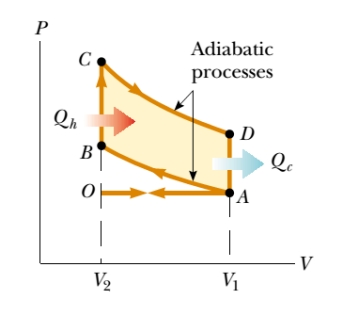
\includegraphics[width=5cm,height=5cm]{Chapter7_otto.png}
            \end{center}
            AB与CD为绝热过程,$Q = 0$,我们只需考虑BC过程的吸热与DA过程的放热。
            这是两个等压过程,它们的热为:
            \begin{equation}
                \begin{aligned}
                    &Q_{in} = Q_{BC} = nC_{V}\Delta T_{BC}= nC_{V}(T_{C} - T_{B})\\
                    &Q_{out} = -Q_{DA} = -nC_{V}\Delta T_{DA}= nC_{V}(T_{D} - T_{A})
                \end{aligned}
                \nonumber
            \end{equation}
            那么有热机效率:
            \begin{equation}
                e = \frac{Q_{in}-Q_{out}}{Q_{in}} = 1 - \frac{T_{D} - T_{A}}{T_{C} - T_{B}}
            \end{equation}
        \end{prove}
        \begin{prove}[Efficiency of a Carnot Cycle]
            这和奥托循环的证明几乎一样

            卡诺循环如下:
            \begin{center}
                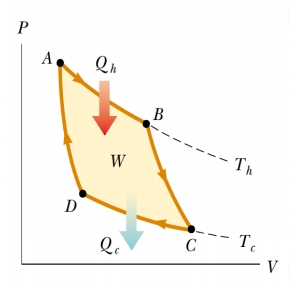
\includegraphics[width=5cm,height=5cm]{Chapter7_carnot.png}
            \end{center}
            AB与CD为绝热过程,$Q = 0$,我们只需考虑AB过程的吸热与CD过程的放热。
            这是两个等温过程,它们的热为:
            \begin{equation}
                \begin{aligned}
                    &Q_{in} = Q_{AB} = nRT_{h}\ln\frac{V_B}{V_A}\\
                    &Q_{out} = -Q_{CD} = nRT_{c}\ln\frac{V_C}{V_D}
                \end{aligned}
                \nonumber
            \end{equation}
            绝热过程有:
            \begin{equation}
                P_{C}V_{C}^{\gamma} = P_{B}V_{B}^{\gamma} \qquad   P_{A}V_{A}^{\gamma} = P_{D}V_{D}^{\gamma}
                \nonumber
            \end{equation}
            而根据理想气体定律$PV=nRT$,得到绝热过程温度与体积的关系:
            \begin{equation}
                T_{c}V_{C}^{\gamma-1} = T_{h}V_{B}^{\gamma-1} \qquad T_{c}V_{D}^{\gamma-1} = T_{h}V_{A}^{\gamma-1}
                \nonumber
            \end{equation}
            那么两式左右分别对应相除,易得:
            \begin{equation}
                \frac{V_C}{V_D} = \frac{V_B}{V_A}
                \nonumber
            \end{equation}
            那么有热机效率:
            \begin{equation}
                e = \frac{Q_{in}-Q_{out}}{Q_{in}} = 1 - \frac{T_{c}}{T_{h}}
            \end{equation}
        \end{prove}
        \section{Part 2}
        \begin{prove}[Boltzmann Distribution]
            虽然笔记主体先给出麦克斯韦分布,然后利用其结论进行玻尔兹曼分布的推导,但实际上顺序是有问题的,下面给出事实上的推导过程。

            首先需要了解,在经典体系中,粒子被认为是\textbf{可辨的},即每个粒子都被认为是不同的对象;
            将所有微观粒子排布到能级(假设每个能级所能容纳的粒子是无限的)上,产生一种\textbf{微观态}。
            这些微观态中,所有对应能级上粒子数均相同的微观态属于同一个\textbf{分布};而这些分布中出现概率最大的,称为\textbf{最概然速率}

            接着是一个统计力学的基本假设,由玻尔兹曼提出:处在平衡的孤立系统,其每个微观态的出现概率是\textbf{相等的}。

            由于宏观态事实上是所有微观态的叠加,其能级分布是各分布的叠加,而最概然分布对其中贡献最大,可以认为宏观分布就是最概然分布。
            有了这些知识和这个前提,我们来推导最概然分布。

            假设有$N$个粒子以及$k$个能级,第$i$个能级的简并度为$w_i$。先考虑向第1个能级填入$a_1$个粒子,这相当于先从$N$个粒子中选出$a_1$个,
            然后将每个粒子可以填入$w_1$个简并轨道中的其中任意一个,对应的情况总共有:
            \begin{equation}
                \Omega_1 =C_{a_1}^{N} (w_1)^{a_1} = \frac{N!}{a_{1}!(N-a_{1})!} (w_1)^{a_1}
            \end{equation}
            然后粒子数变为$N-a_1$,用同样的方法考虑第2个能级,得到:
            \begin{equation}
                \Omega_2 =C_{a_2}^{N-a_1} (w_2)^{a_2} = \frac{(N-a_1)!}{a_{2}!(N-a_{1}-a_{2})!} (w_2)^{a_2}
            \end{equation}
            以此类推,并将所有可能数相乘,得到分布数:
            \begin{equation}
                \Omega = \prod_{i=1}^{k} \Omega_{i} = \frac{N!}{\prod_{i = 1}^{k}a_{i}!}\prod_{i = 1}^{k} (w_i)^{a_i}
            \end{equation}
            因为对数与原函数在同一点取极值,所以我们对它取个对数,有:
            \begin{equation}
                \ln\Omega = \ln(N!)\sum_{i = 1}^{k}[{a_i}\ln(w_i) - \ln(a_i!)]
            \end{equation}
            $N$是一个很大的数,我们假设所有的$a_i$也是很大的数\footnote{这一假设对真实气体并不严谨,但推导理想气体够用了},
            使用如下的积分估值:
            \begin{equation}
                \ln(N!) = \ln(\prod_{i=1}^{N}i)=\sum_{i=1}^{N}\ln(i) \approx \int_{1}^{N}\ln x\dif{x} = N\ln N-N
            \end{equation}
            并且注意到$\sum_{i=1}^{k}a_i=N$,就可以得到:
            \begin{equation}
                \begin{aligned}
                    \ln\Omega &= N\ln N-N-\sum_{i=1}^{k}a_{i}\ln(a_i)+\sum_{i=1}^{k}a_k+\sum_{i = 1}^{k}{a_i}\ln(w_i)\\
                    &=N\ln N-\sum_{i=1}^{k}a_{i}\ln(a_i)+\sum_{i = 1}^{k}{a_i}\ln(w_i)
                    \label{of_omega}
                \end{aligned}
            \end{equation}
            全微分:
            \begin{equation}
                \dif{(\ln\Omega)} = \sum_{i=1}^{k}\left(\frac{\partial (\ln\Omega)}{\partial a_i}\right)_{a_j(i\neq j)} \dif{a_i} = 
                -\sum_{i=1}^{k}(1+\ln a_i-\ln w_i)\dif{a_i} 
                \label{of_difOmega}
            \end{equation}
            考虑存在如下两个约束条件,所有能级上的粒子之和等于$N$,所有粒子的能量之和等于内能$U$,设第$i$个能级的能量为$\epsilon_i$,即有:
            \begin{equation}
                \begin{aligned}
                    &\sum_{i=1}^{k}a_i = N\\
                    &\sum_{i=1}^{k}a_i \epsilon_i = U
                    \label{of_U}
                \end{aligned}
            \end{equation}
            要求极值,显然使用拉格朗日乘因子法,分别对上式微分后乘以$\alpha + 1$,$\beta$加到\ref{of_difOmega}中,可得到:
            \begin{equation}
                \sum_{i=1}^{k} [\ln(\frac{w_i}{a_i})+\alpha+\beta \epsilon_i] \dif{a_i} = 0
            \end{equation}
            此时变量相互独立,只需令每一项均为0即可,得到:
            \begin{equation}
                \ln(\frac{w_i}{a_i})+\alpha+\beta \epsilon_i = 0
                \label{of_a_i}
            \end{equation}
            写成指数形式也就是:
            \begin{equation}
                a_i = w_i e^{\alpha + \beta \epsilon_i}
                \label{of_a_i_2}
            \end{equation}

            下面我们更进一步,来试试把$\alpha$与$\beta$的表达式求出来。

            我们现在重新观察一下\ref{of_omega},并将其写成如下形式:
            \begin{equation}
                \ln\Omega = N\ln N + \sum_{i = 1}^{k} a_i \ln(\frac{w_i}{a_i})
            \end{equation}
            这样我们较为方便的把\ref{of_a_i}代入,并注意一下\ref{of_U},不难得到:
            \begin{equation}
                \ln\Omega = N\ln N - \alpha \sum_{i = 1}^{k} a_i -\beta \sum_{i = 1}^{k}\epsilon_i a_i = N\ln N -\alpha N - \beta U  
            \end{equation}
            接着我们利用熵的微观表达式,即玻尔兹曼公式,并结合最概然分布的假设,代入有:
            \begin{equation}
                S = k_{_B}\ln\sum \Omega_i = k_{_B}\ln\Omega =  k_{_B}N\ln N -k_{_B}\alpha N - k_{_B}\beta U
                \label{of_S}
            \end{equation}
            最后结合温度的定义即可求得$\beta$:
            \begin{equation}
                \begin{aligned}
                    &\frac{\partial S}{\partial U} = -k_{_B}\beta =\frac{1}{T}\\
                    &\beta = -\frac{1}{k_{_B}T}
                \end{aligned}
            \end{equation}
            定义配分函数如下:
            \begin{equation}
                Z \overset{def}{=} \sum_{i=1}^{k}w_i e^{-\tfrac{\epsilon_i}{k_{_B}T}}
            \end{equation}
            将\ref{of_a_i_2}代入\ref{of_U}的$N$中,可以得到:
            \begin{equation}
                \begin{aligned}
                    &N = Ze^{\alpha} \\
                    &\alpha = \ln\left(\frac{N}{Z}\right)
                \end{aligned}
            \end{equation}
            就有了最基本的形式:
            \begin{equation}
                a_i = \frac{w_{i}N}{Z} e^{-\tfrac{\epsilon_i}{k_{_B}T}}
                \label{of_a_i_3}
            \end{equation}
            设第一个能级为基态,其能量为0(由于习惯,基态用下标“0”表示),且能级无简并($w_i=1$):
            \begin{equation}
                a_{_0} = e^{\alpha}
            \end{equation}
            从而得到有:
            \begin{equation}
                a_i = a_{_0} e^{-\tfrac{\epsilon_i}{k_{_B}T}} 
            \end{equation}
            这样我们就得到了玻尔兹曼分布的表达式。
        \end{prove}
        \begin{prove}[Maxwell Distribution]            
            想象速度的分布表示在三维坐标系中,也就是速度空间,向$x$,$y$,$z$坐标分别表示$v_x$,$v_y$,$v_z$,速度相同的粒子分布在同一点。
            在这样一个空间中,我们来考察速度在$v$到$v+\dif{v}$的粒子,相当于不计速度方向而考虑速度大小,那么它所覆盖的体积显然是一个厚度为$\dif{v}$的球壳。
            它的体积为:
            \begin{equation}
                \dif{V} = \frac{4}{3}\pi (\dif{v}+v)^{3} - \frac{4}{3}\pi v^{3} = 4\pi v^{2}\dif{v} + o(\dif{v}) = 4\pi v^{2}\dif{v}
            \end{equation}
            根据玻尔兹曼分布\ref{of_a_i_3},在这个速度的粒子数密度与动能的关系为
            \footnote{这里我们不考虑能级简并问题,因为经典动能是连续的,导致了对$v_{x}^{2}+v_{y}^{2}+v_{z}^{2}=A$来说,
            在$A>0$的情况下总是有无数组解。}:
            \begin{equation}
                a= \frac{N}{Z} e^{-\tfrac{\mu v^{2}}{2k_{_B}T}}
            \end{equation}
            下面来求配分函数,在连续空间中,我们把累加化为积分。因为位置和速度都可能影响能级能量
            \footnote{虽然这里的空间分布不影响能量,但不代表积分时可以不考虑。}
            ,所以积分区间应遍历整个空间与速度空间,即相空间:
            \begin{equation}
                Z =\int \dots \int e^{-\tfrac{\mu v^{2}}{2k_{_B}T}} \dif{x}\dif{y}\dif{z}\dif{v_x}\dif{v_y}\dif{v_z}
            \end{equation}
            注意到能量与空间分布无关,所以对空间的积分就等于$V$,然后看对速度的积分,由于只需考虑速度大小且积分区间为全速度空间,
            我们选择从球壳逐层积分,即$\dif{v_x}\dif{v_y}\dif{v_z} = 4\pi v^{2}\dif{v}$,从而:
            \begin{equation}
                \begin{aligned}
                    Z &= 4\pi V\int_{0}^{+\infty} v^{2} e^{-\tfrac{\mu v^{2}}{2k_{_B}T}} \dif{v}\\
                      &= -\frac{4 \pi V k_{_B}T}{\mu} (ve^{-\tfrac{\mu v^{2}}{2k_{_B}T}}\big|_{0}^{+\infty} - \int_{0}^{+\infty} e^{-\tfrac{\mu v^{2}}{2k_{_B}T}} \dif{v})
                \end{aligned}
            \end{equation}
            前一项显然为0,后一项是经典的高斯积分,在概率论与数学分析中都有涉及它的求解,这里直接给出结果:
            \begin{equation}
                Z = \frac{4 \pi V k_{_B}T}{\mu} (\frac{1}{2}\sqrt{\frac{2\pi k_{_B}T}{\mu}}) = V\left(\frac{2\pi k_{_B}T}{\mu}\right)^{\frac{3}{2}}
                \label{of_Z}
            \end{equation}
            将它代入粒子数的表达式,我们可以得到粒子密度随动量的分布:
            \begin{equation}
                \rho = \frac{a}{V} = N\left(\frac{\mu}{2\pi k_{_B}T}\right)^{\frac{3}{2}}e^{-\tfrac{\mu v^{2}}{2k_{_B}T}}
            \end{equation}
            这样就可以求$\dif{N}$了,它等于速度空间体积元内的粒子数:
            \begin{equation}
                \dif{N} = \rho \dif{V} = N4\pi \left(\frac{\mu}{2\pi k_{_B}T}\right)^{\frac{3}{2}}v^{2}e^{-\tfrac{\mu v^{2}}{2k_{_B}T}}\dif{v}
            \end{equation}
            联系速率分布函数的定义,其实我们已经得到了麦克斯韦分布:
            \begin{equation}
                f(v) = \frac{\dif{N}}{N\dif{v}} = 4\pi \left(\frac{\mu}{2\pi k_{_B}T}\right)^{\frac{3}{2}}v^{2}e^{-\tfrac{\mu v^{2}}{2k_{_B}T}}
            \end{equation}
            证毕。
        \end{prove}
        \begin{prove}[Ideal Gas Law]
            先回到玻尔兹曼分布\ref{of_S},我们已经求出了这里的$\alpha$与$\beta$,直接代入:
            \begin{equation}
                S = k_{_B}N\ln N - k_{_B}N\ln\frac{N}{Z} + \frac{U}{T} = k_{_B}N\ln Z + \frac{U}{T}
            \end{equation}
            定义亥姆霍兹自由能$A=U-TS$,从而上式化为:
            \begin{equation}
                A = -k_{_B}NT\ln Z
            \end{equation}
            这里的配分函数我们已经计算过了,直接代入\ref{of_Z}
            \footnote{严谨来说应该把外势场以及转动动能考虑进去,不过那样配分函数还是$Z=\ln(Vf(T))$的形式,区别只是$f(T)$不影响推导}:
            \begin{equation}
                A = -k_{_B}NT\ln\left[V\left(\frac{2\pi k_{_B}T}{\mu}\right)^{\frac{3}{2}}\right]
                \label{of_A}
            \end{equation}
            代入热力学基本方程$dU=T\dif{S}-p\dif{V}$,可以得到
            \footnote{事实上热力学基本方程有四个,这也被视为其中一个,还有两个分别关于焓$H$与吉布斯自由能$G$}:
            \begin{equation}
                \dif{A} = -S\dif{T} - p\dif{V}
                \label{of_dif_A}
            \end{equation}
            $A$为状态函数,上式是全微分,所以:
            \begin{equation}
                \left(\frac{\partial A}{\partial V}\right)_{T} = -p
            \end{equation}
            代入$A$有:
            \begin{equation}
                \left(\frac{\partial A}{\partial V}\right)_{T} = -\frac{k_{_B}NT}{V} =-p
            \end{equation}
            这就是理想气体定律,重写为:
            \begin{equation}
                pV = Nk_{_B}T
            \end{equation}
            证毕。
        \end{prove}
        \begin{prove}[Equipartition Theorem]
            首先考虑最简单的单原子分子,其只有平动动能,故其$A$与\ref{of_A}一致,结合\ref{of_dif_A},得到熵的表达式:
            \begin{equation}
                \begin{aligned}
                    S &= -\left(\frac{\partial A}{\partial T}\right)_{V} \\
                      &= k_{_B}N\ln\left[V\left(\frac{2\pi k_{_B}T}{\mu}\right)^{\frac{3}{2}}\right]+\frac{3}{2}k_{_B}N\\
                      &= -\frac{A}{T} +\frac{3}{2}k_{_B}N
                \end{aligned}
            \end{equation}
            由$U=A+ST$即得到:
            \begin{equation}
                U = \frac{3}{2}k_{_B}NT = \frac{3}{2}RT
            \end{equation}
            这与单原子分子只有三个平动自由度相吻合。
            
            然后把转动动能考虑进来,先来看非线性分子。令$I=\frac{1}{2}Jw^{2}$为转动动能,取类似于速度空间的角速度空间,这样考虑了转动后的配合函数变为:
            \begin{equation}
                Z =\int \dots \int e^{-\tfrac{\mu v^{2}+J w^{2}}{2k_{_B}T}} \dif{x}\dif{y}\dif{z}\dif{v_x}\dif{v_y}\dif{v_z}\dif{w_x}\dif{w_y}\dif{w_z}
            \end{equation}
            由于非线性分子实际上平动动能与转动动能形式一致,故积分结果也一致,有:
            \begin{equation}
                Z =  V\left(\frac{4\pi^{2} k_{_B}^{2}}{\mu J}\right)^{\frac{3}{2}} T^{3}
            \end{equation}
            经过与前面相同的推导可以得到:
            \begin{equation}
                U = 3k_{_B}NT = 3RT
            \end{equation}
            到这里已经可以发现,平动与转动自由度影响了配分函数对温度的次数,后者与内能对$RT$的系数一致。

            对线性分子,绕穿过分子的那条轴的转动惯量过小,对应方向上的转动动能可以忽略。
            假设忽略$w_z$,则体积元从球壳变为圆柱体壳,即$\dif{w_x}\dif{w_y}\dif{w_z}=2\pi w\dif{w}$,即下面的积分:
            \begin{equation}
                2\pi \int_{0}^{+\infty} we^{-\tfrac{J w^{2}}{2k_{_B}T}}\dif{w} = \frac{2\pi k_{B}T}{J}
            \end{equation}
            于是有$Z\propto T^{\frac{5}{2}}$,对应的:
            \begin{equation}
                U = \frac{5}{2}k_{_B}NT = \frac{5}{2}RT
            \end{equation}
            必须指出,我们用积分计算配分函数意味着我们假设平动能级和转动能级的能隙相对于$k_{_B}T$来说很小,
            所以把能级近似为连续的考虑。这一假设对于振动能级开始已经不再成立,我们必须使用求和代替积分,这个计算出来的贡献相对前两者来说可以忽略,
            不过这部分的计算需要使用量子力学,这里就不给出振动贡献可忽略的证明了。
        \end{prove}
%\end{document}
